\documentclass[10pt,twocolumn]{article}
\usepackage[a4paper,margin=20mm,columnsep=7mm]{geometry}
\usepackage{times}
\usepackage{graphicx}
\usepackage{amsmath}
\usepackage{booktabs}
\usepackage{xcolor}
\usepackage[hidelinks]{hyperref}
\usepackage{microtype}
\usepackage{caption}
\captionsetup{font=small,labelfont=bf}
\setlength{\parskip}{2pt}

\title{\vspace{-6mm}Ask Them or Test Them? Persona Polling Predicts the Opposite of Behavioural Replication in LLM Simulation of a UK Food-Labelling Trial\\[2mm]\large A pilot study}
\author{Emily Kelt\thanks{University of Cambridge. \texttt{emk50@cam.ac.uk}. Code, data pipeline and all raw model outputs: project repository \texttt{simulated societies}. Draft of 22 October 2026.}}
\date{}

\begin{document}
\maketitle

\begin{abstract}
Commercial ``synthetic respondent'' tools predict how an audience will react to a message by prompting language-model personas and asking them which message would change their behaviour. We test this design against an open randomised experiment with a behavioural outcome: Clarke et al.\ (2020), in which 4,134 UK adults chose a snack from a simulated vending machine under one of six labelling conditions. Using the same interview-grounded personas, the same models and the same human data, we compare \emph{asking} personas which labelling scheme would move them with \emph{placing} each persona in one arm of the experiment and recording its choice. The two designs disagree in sign. Across three Claude models, polled personas consistently favoured calorie badges and dismissed graphic health warnings, the reverse of the human result; placed in the experiment, Claude Sonnet~5.5 reproduced the human ordering of the six arms in every demographic segment (mean segment-level Spearman $\rho = 0.79$, bootstrap 95\% CI $[0.66, 0.80]$, against a pooled-population baseline of $0.82$). Two cheaper models, Claude Haiku~5.5 and Haiku~4.5, collapsed to choosing an energy-dense snack in 94--97\% of trials regardless of condition, and a single deleted prompt sentence moved Haiku~5.5's accuracy from $0.33$ to $0.47$. An adversarial-critic ``debate'' round changed answers substantially but did not improve accuracy. We also find a three-fold inflation of the education gap by the best model. The results are from one dataset at pilot scale and should be read as hypotheses, but they argue that audience-simulation tools should replicate the decision, not poll the persona, and should report a human noise ceiling alongside any segment-level claim.
\end{abstract}

\section{Introduction}
A growing market (Aaru, Artificial Societies, Simile, Qualtrics Edge Audiences, Toluna, YouGov/Yabble) sells LLM ``digital twins'' that forecast how population segments will respond to marketing or public-health messages before any human sees them. The academic evidence is mixed. Conditioned on rich backstories, LLMs reproduce group-level survey distributions reasonably well \cite{argyle2023,park2024}, and aggregated LLM forecasts of survey-experiment treatment effects correlate at $r \approx 0.85$--$0.90$ with realised effects \cite{hewitt2024,lippert2024}. Yet the same models flatten within-group variance, drift toward socially desirable answers, inflate between-group differences two- to four-fold, and are sensitive to cosmetic prompt changes \cite{wang2024,bisbee2024,salecha2024,chen2026fail}. Nearly all of this evidence concerns survey items. Message testing is different: the outcome of interest is what people \emph{do} after exposure, and the human literature has long known that people are poor at reporting what persuades them, especially for fear appeals \cite{witte2000}.

This note asks a narrow question. Holding personas, models and ground truth fixed, does it matter whether the simulator \emph{asks} the persona which message would work, or \emph{tests} the persona by placing it in the experiment? We also ask whether cheap models suffice, and whether an adversarial critic round helps.

\section{Method}
\paragraph{Ground truth.} Clarke et al.\ \cite{clarke2020} randomised 4,134 UK adults to one of six labelling conditions in a $3\times 2$ design (health warning: pictorial, text-only, none; calorie badge: present, absent) and asked them to pick one of twelve snacks, six energy-dense, from a hypothetical vending machine. The primary outcome is whether an energy-dense snack was chosen. Individual-level age, gender, ethnicity, education and BMI are released on OSF (\texttt{k7tw5}). We define arm effectiveness as $1 - P(\text{energy-dense})$ and compute it for eight segments: gender $\times$ age band (18--34, 35--54, 55+) and education (degree, no degree). Two reference points are computed from the human data alone: the \emph{pooled baseline}, the Spearman correlation obtained by predicting every segment with the whole-population ranking ($0.82$ for gender$\times$age, $0.94$ for education), and a \emph{split-half ceiling}, the mean correlation between segment rankings computed on two random halves of the human sample ($0.60$ and $0.88$). The ceiling bounds what any method can achieve; the baseline is what segmentation must beat to add value.

\paragraph{Personas.} For each segment we generate 8--12 personas. Each is a $\sim$250-word first-person interview transcript written by the model under test, constrained to the segment's demographics plus three randomly drawn mundane life facts (shift work, shops at the corner shop, sceptical of government advice, \dots) to induce within-segment variation. Interview-style grounding follows \cite{park2024,lutz2025}. A \emph{label} condition uses the bare demographic description instead.

\paragraph{Elicitation designs.} All designs see the same six arm descriptions in randomised order.
\begin{itemize}\setlength{\itemsep}{0pt}
\item \textbf{Poll (points).} The persona allocates 100 points across the six labelling schemes ``in proportion to how much each would actually change what you buy''. Variants: a single grounded persona sampled five times; a crowd of 12 independent grounded personas; a label-only persona; and a no-persona \emph{judge} in which the model, as a communication expert, predicts the segment.
\item \textbf{Poll + critic (debate).} After the crowd answers, a ``blunt friend from the same community'' critiques each answer and the persona revises. Adversarial rather than consensus-seeking, since consensus debate is known to homogenise \cite{smit2024,debatevote2025}.
\item \textbf{Replicate (choice).} Each persona is placed in \emph{one} arm, shown the twelve snacks with that arm's labelling, and asked to pick the one it would take now. Two draws per persona per arm; effectiveness is the share of lower-energy choices. This is the between-subjects design of the original trial, in the spirit of ``Turing experiments'' \cite{aher2023}.
\end{itemize}

\paragraph{Models and cost.} Claude Sonnet~5.5 (\$2/\$10 per M tokens), Haiku~5.5 (\$0.10/\$0.50) and Haiku~4.5 (\$1/\$5), temperature 1, thinking effort low. Total spend for every result reported here was about \$9. Non-Anthropic low-cost models are supported by the pipeline but were not run.

\paragraph{Metrics.} Mean Spearman correlation between predicted and human rankings of the six arms within each segment; top-1 accuracy (did the method pick the human-best arm); gap preservation, the Pearson correlation between predicted and human between-segment differences, arm by arm; and 95\% bootstrap intervals over personas (1,000 resamples).

\begin{table*}[t]
\centering\small
\caption{Study 2 of Clarke et al.\ (2020). Segment-level mean Spearman $\rho$ against human arm rankings (bootstrap 95\% CI over personas), top-1 accuracy, between-segment gap preservation, and the population-level ordering correlation. Human reference points: pooled baseline $0.82$ / $0.94$, split-half ceiling $0.60$ / $0.88$ (gender$\times$age / education).}
\label{tab:main}
\begin{tabular}{llcccccr}
\toprule
Model & Design & $\rho$ (segment) & 95\% CI & top-1 & gap & $\rho$ (pooled) & cost \\
\midrule
Sonnet 5.5 & Replicate (choice) & \textbf{0.79} & [0.66, 0.80] & \textbf{0.62} & \textbf{0.36} & 0.94 & \$2.10 \\
Sonnet 5.5 & Judge, no persona & 0.78 & [0.71, 0.79] & 0.38 & 0.14 & 0.89 & \$0.32 \\
Sonnet 5.5 & Poll, label persona & 0.41 & [0.35, 0.47] & 0.38 & $-0.17$ & -- & \$0.22 \\
Sonnet 5.5 & Poll, grounded crowd (12) & 0.20 & [0.17, 0.27] & 0.00 & 0.08 & 0.26 & \$0.42 \\
Sonnet 5.5 & Poll + critic & 0.26 & [0.21, 0.35] & 0.00 & 0.28 & 0.26 & \$0.89 \\
\midrule
Haiku 5.5 & Replicate (choice) & 0.33 & [0.05, 0.52] & 0.12 & 0.03 & 0.75 & \$0.26 \\
Haiku 5.5 & Replicate, neutral prompt & 0.47 & [0.24, 0.57] & 0.50 & 0.37 & 0.89 & \$0.28 \\
Haiku 5.5 & Judge, no persona & 0.29 & [0.19, 0.36] & 0.12 & $-0.13$ & 0.26 & \$0.02 \\
Haiku 5.5 & Poll, label persona & 0.12 & [$-0.01$, 0.28] & 0.00 & 0.08 & -- & \$0.02 \\
Haiku 5.5 & Poll, grounded crowd (12) & $-0.37$ & [$-0.46$, $-0.26$] & 0.00 & 0.10 & $-0.60$ & \$0.05 \\
Haiku 5.5 & Poll + critic & $-0.36$ & [$-0.46$, $-0.15$] & 0.00 & $-0.07$ & $-0.43$ & \$0.10 \\
\midrule
Haiku 4.5 & Replicate (choice) & $-0.17$ & [$-0.37$, 0.07] & 0.12 & $-0.01$ & 0.09 & \$1.17 \\
Haiku 4.5 & Judge, no persona & 0.40 & [0.26, 0.48] & 0.25 & $-0.10$ & 0.49 & \$0.14 \\
Haiku 4.5 & Poll, grounded crowd (12) & $-0.38$ & [$-0.52$, $-0.20$] & 0.00 & $-0.03$ & $-0.60$ & \$0.25 \\
Haiku 4.5 & Poll + critic & 0.01 & -- & 0.25 & 0.13 & -- & \$0.53 \\
\bottomrule
\end{tabular}
\end{table*}

\section{Results}

\paragraph{Polling personas gets the sign wrong.} Figure~\ref{fig:stated} shows the core result. Asked which labelling scheme would change their behaviour, Sonnet's grounded crowd put 36\% of its points on calorie badges alone and 5\% on pictorial warnings; humans chose a lower-energy snack 46\% of the time under calorie badges and 63\% under pictorial warnings. The rationales are recognisably human: ``gory pictures would make me roll my eyes'', ``a number I can take in at a glance''. Both Haiku models produce the same pattern, with population-level correlations of $-0.60$. The poll design is not noisy; it is confidently wrong in a direction the fear-appeal literature predicts for self-report \cite{witte2000}.

\paragraph{Replicating the experiment recovers the human ordering, on one model.} Placed inside the trial, Sonnet~5.5 reproduced the human ordering (pictorial $>$ text $>$ calories $>$ nothing) in all eight segments (Figure~\ref{fig:arms}), with segment-level $\rho = 0.79$ and top-1 accuracy $0.62$. This matches the pooled-population baseline and exceeds the gender$\times$age noise ceiling; it does not show that segmentation adds information beyond the population ranking, and in this dataset there is little such information to add. A no-persona Sonnet judge reaches almost the same rank accuracy ($0.78$) at a sixth of the cost, but with weaker gap preservation ($0.14$ vs $0.36$).

\begin{figure}[t]
\centering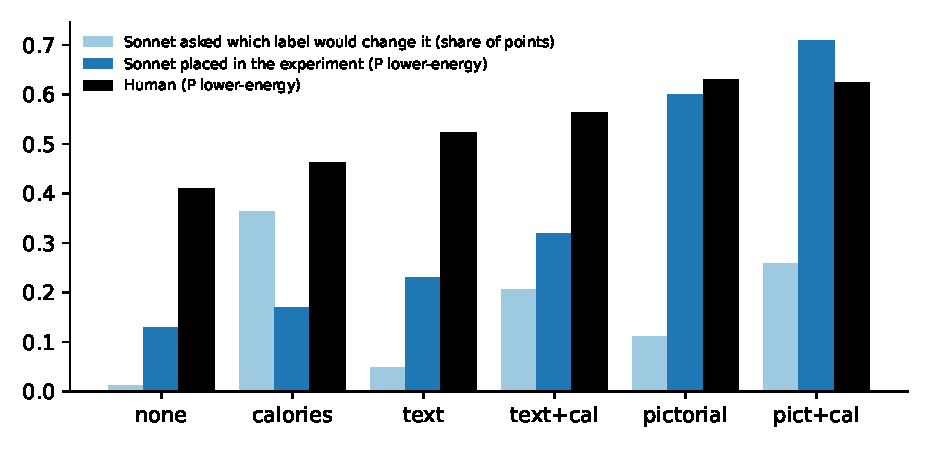
\includegraphics[width=\columnwidth]{fig_stated_revealed.pdf}
\caption{Same model (Sonnet~5.5), same personas, opposite conclusions. Light bars: share of 100 points the polled crowd gave each labelling scheme. Dark bars: share of lower-energy choices when personas were placed in each arm. Black: human participants.}
\label{fig:stated}
\end{figure}

\begin{figure}[t]
\centering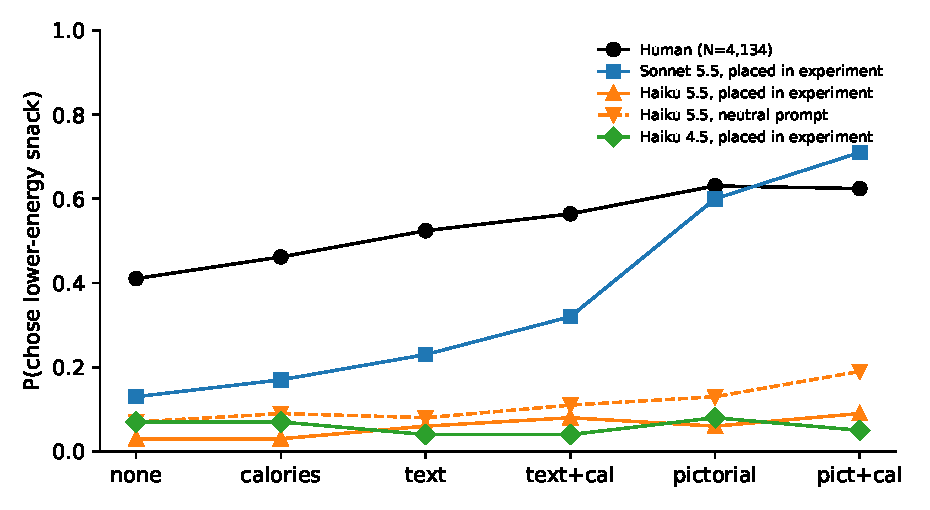
\includegraphics[width=\columnwidth]{fig_arms.pdf}
\caption{Population-level share of lower-energy snack choices by arm. Sonnet reproduces the human ordering with exaggerated spread. Both Haiku models sit near zero in every arm; removing one sentence from the prompt (dashed) more than doubles Haiku~5.5's rate.}
\label{fig:arms}
\end{figure}

\paragraph{Cheap models collapse rather than err.} Haiku~5.5 and 4.5 personas chose an energy-dense snack in 94--97\% of trials in every arm; humans did so in 59\% of control trials. With almost no variance there is nothing to rank, and the between-model difference in $\rho$ is mostly noise around a floor. The collapse is prompt-dependent: deleting the sentence ``Do not try to be healthy or make a point'' raised Haiku~5.5's lower-energy rate from $0.07$ to $0.19$ and its segment-level $\rho$ from $0.33$ to $0.47$, with the population-level ordering rising to $0.89$. A change that should be semantically neutral moved the estimate more than the treatment did, as \cite{bisbee2024} found for survey items.

\paragraph{The best model over-determines demographics.} Sonnet placed the no-degree segment at $0.1$--$0.3$ lower-energy choices and the degree segment at $0.3$--$0.9$; the human figures are $0.36$--$0.62$ and $0.44$--$0.66$. The direction is right and the magnitude is roughly three times too large, consistent with the $2$--$4\times$ gap inflation reported by \cite{chen2026fail}. Any segment difference shown to a user needs shrinkage calibrated on a human pilot.

\paragraph{An adversarial critic moves answers but not accuracy.} The critic round shifted 17--29 points per persona and slightly increased within-segment variance (Sonnet: SD $5.1 \to 5.9$), so it is not a consensus-collapse mechanism. Rank accuracy was unchanged (Sonnet $0.20 \to 0.26$; Haiku~5.5 $-0.37 \to -0.36$) at two to three times the cost. A critic cannot repair an elicitation whose signal is wrong-signed.

\paragraph{Null check.} Study 1 of the same project (4,607 adults rating desire for a chocolate bar under six disease framings) has a split-half ceiling of $0.17$: humans barely distinguish the framings. Haiku~5.5 methods scored $0.17$--$0.38$, consistent with noise, yet every method produced a confident ``best framing'' per segment. A simulator that does not report the ceiling will present noise as insight.

\section{Discussion}
The practical recommendation is simple: simulate the decision, not the opinion about the decision. This is how the strongest published results were obtained \cite{hewitt2024,aher2023}, and it is the opposite of how most persona-polling products are used. Three caveats bound the claim. First, one dataset with modest true heterogeneity; the two open datasets with published heterogeneity, label design by Latino parents \cite{hall2021} and climate labels by sex \cite{wolfson2022}, need author requests. Second, pilot scale: 8--12 personas per cell and two draws, where $\sim$200 draws per cell are recommended for stable distributions \cite{sun2024}. Third, one prompt wording per design; the Haiku ablation shows that any number here is partly a property of the prompt. A full study would run three datasets, four model families including open-weight and base models \cite{lutz2025}, five paraphrases per design, and report each model as a distribution over wordings.

\section{Conclusion}
On an open behavioural trial, asking LLM personas which public-health message would move them predicted the reverse of what people did, while placing the same personas in the experiment reproduced the human ordering with a capable model. Cheap models collapsed, a critic round did not help, and segment gaps were inflated. Audience-simulation tools should replicate decisions, calibrate segment gaps on human pilots, and publish the human noise ceiling with every prediction.

\small
\begin{thebibliography}{99}\setlength{\itemsep}{0pt}
\bibitem{aher2023} Aher, G., Arriaga, R., Kalai, A. (2023). Using large language models to simulate multiple humans and replicate human subject studies. ICML. arXiv:2208.10264.
\bibitem{argyle2023} Argyle, L.\ et al.\ (2023). Out of one, many: Using language models to simulate human samples. \emph{Political Analysis} 31(3).
\bibitem{bisbee2024} Bisbee, J.\ et al.\ (2024). Synthetic replacements for human survey data? The perils of large language models. \emph{Political Analysis}.
\bibitem{chen2026fail} Chen, Zhu, Zheng (2026). When synthetic users fail. arXiv:2607.26348.
\bibitem{clarke2020} Clarke, N., Pechey, E., Mantzari, E.\ et al.\ (2020). Impact of health warning labels on snack selection: An online experimental study. \emph{Appetite}. Data: \url{https://osf.io/k7tw5/}.
\bibitem{debatevote2025} Debate or vote: Which yields better decisions in multi-agent large language models? (2025). arXiv:2508.17536.
\bibitem{hall2021} Hall, M.\ G., Lazard, A.\ J., Grummon, A.\ H.\ et al.\ (2021). Designing warnings for sugary drinks: A randomized experiment with Latino and non-Latino parents. \emph{Preventive Medicine} 148.
\bibitem{hewitt2024} Hewitt, L., Ashokkumar, A., Ghezae, I., Willer, R. (2024/2026). Predicting results of social science experiments using large language models. \emph{Nature}.
\bibitem{lippert2024} Lippert, S.\ et al.\ (2024). Can large language models help predict results from a complex behavioural science study? \emph{Royal Society Open Science}.
\bibitem{lutz2025} Lutz, Sen, Ahnert, Rogers, Strohmaier (2025). The prompt makes the person(a). Findings of EMNLP. arXiv:2507.16076.
\bibitem{park2024} Park, J.\ S.\ et al.\ (2024). Generative agent simulations of 1,000 people. arXiv:2411.10109.
\bibitem{salecha2024} Salecha, A.\ et al.\ (2024). Large language models display human-like social desirability biases in Big Five personality surveys. \emph{PNAS Nexus}.
\bibitem{smit2024} Smit, A.\ et al.\ (2024). Should we be going MAD? A look at multi-agent debate strategies for LLMs. ICML.
\bibitem{sun2024} Sun, S.\ et al.\ (2024). Random silicon sampling. arXiv:2402.18144.
\bibitem{wang2024} Wang, A., Morgenstern, J., Dickerson, J.\ (2024). Large language models should not replace human participants because they can misportray and flatten identity groups. arXiv:2402.01908.
\bibitem{witte2000} Witte, K., Allen, M.\ (2000). A meta-analysis of fear appeals: Implications for effective public health campaigns. \emph{Health Education \& Behavior} 27(5).
\bibitem{wolfson2022} Wolfson, J.\ A.\ et al.\ (2022). Effect of climate change impact menu labels on fast food ordering choices. \emph{JAMA Network Open} 5(12).
\end{thebibliography}
\end{document}
